\chapter{IoT}
Sempre più spesso si parla di Internet delle cose o IoT, con questo termine si
intende un evoluzione delle applicazioni legate al settore mobile, al settore
della home automation e al settore embedded.  In questo scenario ogni oggetto
,il quale implementa un sensore al suo interno, disporrà di una connessione ad
Internet.  Avvalendosi di questa connessione , i vari dati raccolti potranno
essere inviati ad un server il quale avrà il compito di elaborarli e fornire
delle applicazioni in grado di adattarsi all'utente finale.  Sebbene il numero
di dispositivi "smart" è in rapida crescita, i servizi che l'IoT offre saranno
il vero valore aggiunto. Aziende e enti pubblici stanno investendo e mettendo a
disposizione sempre più servi in grado di adattarsi, in modo dinamico, a seconda
dati raccolti tramite i vari consumatori . Gartner stima che entro l'anno 2020,
saranno presenti circa 20 miliardi di dispositivi IoT  e  che l'investimento
annuo  in questo settore sarà pari a circa \$5000 milioni di dollari
\cite{gartner2016}. 

\begin{table}[h]
        \centering
        \begin{tabular}{l|c|c|c|c}
                Categoria  & 2016 & 2017 & 2018 & 2019 \\
                \hline
                Consumer  & 3963 & 5244,3 & 7063,3 & 12863 \\
                Business  & 1418 & 2135.4 & 4152,7 & 3171  \\
                Totale    & 6381 & 8380   & 11196  & 20415 \\
        \end{tabular}
        \caption{Stima di dispositivi IoT (Milioni di unità) Gartner\cite{gartner2016}}
\end{table}

In contrasto a tutto ciò, la capacità delle aziende di applicare tecniche di
data analytics, per far fruttare la grande quantità di dati ricevuti, deve ancora
maturare. Secondo un articolo pubblicato da Verizon, si stima che il 92\% delle
aziende usa meno del 25\% dei dati raccolti e che solo il 50\% di esse prevede
di riuscire a fare fruttare più del 25\% di dati nei prossimi due anni \cite{VerizionIoT}


Questa rapida crescita ha portato alla ricerca è sviluppo
di nuove soluzioni tecnologiche per supportare il carico di dispositivi
simultaneamente connessi . Per non alterare il \emph{QoS} Quality of Service ,
hardware e software dovranno essere rivisti insieme alla network topology utilizzata. 
I punti fondamentali sui quali queste tecnologie sono state sviluppate sono: 

\begin{itemize}
\item \textbf{Scalabilità}: Dato l'elevato numero di devices previsti nei scenari
urbani ed industriali, la network technology alla base della rete dovrà essere 
adattabile, in modo dinamico, al carico di dispositivi connessi.
\item \textbf{Costo unitario}: Il costo del end device, dovrà essere conveniente
per garantire la più ampia fetta di mercato.
\item \textbf{Durata della batteria}: La maggior parte dei dispositivi sarà
limentata tramite batteria. Inoltre la ogni devices dovrà garantire una durata
minima dell batteria di circa una decina d'anni. 
\item \textbf{Costo computazionale}: La modulazione, alla base di queste nuove
tipologie di rete, dovrà essere concepita in modo da non richiedere un costo
computazionale elevato .
\item \textbf{Raggio d'azione}: La necessità di utilizzare questi devices in ambienti
difficili o rurali, rende necessario poter instaurare una comunicazione con
devices che si trovano a chilometri di distanza.
\item \textbf{Sicurezza}: Lo scambio dei dati dovrà avvenire in maniera sicura,
implementando algoritmi di cifratura dei dati o procedure di handshaking.
\item \textbf{Tolleranza ai guasti}: Il mal funzionamento  o il guasto di un
nodo della rete,  non dovrà compromettere il funzionamento dell'intera rete a lui connessa. 
\end{itemize}

\begin{figure}[h]
        \centering 
                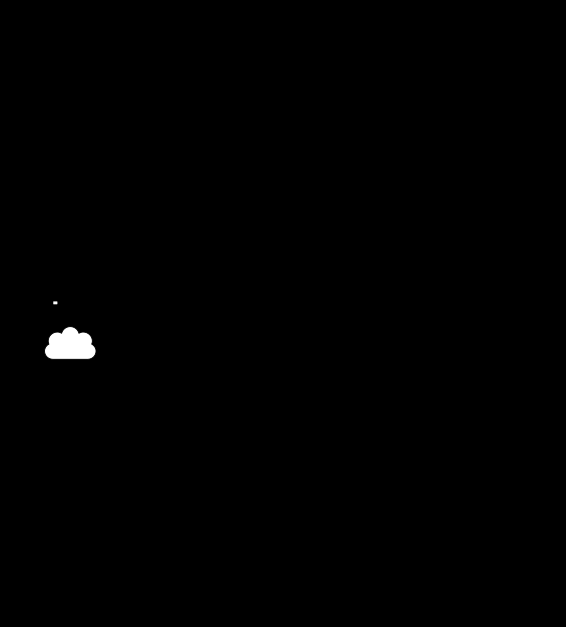
\includegraphics[width=10cm]{three-layer}
        \caption{Layer del IoT}
\end{figure}

Vari tipi di architetture di rete sono stati proposti per realizzare questa
nuova infrastruttura. Per quanto le varie proposte si basano su tecnologie
differenti, è possibile individuare tre layer comuni 
\begin{itemize}
\item \textbf{Device layer} o sensor layer, è il layer più basso. Esso raggruppa
tutti i gli oggetti "smart". Questo layer è quello che mette in comunicazione il
mondo reale con gli atri layer superiori. Esistono diversi tipi di sensori
ognuno con Sensor layer which is the lowest layer consisting of integrated smart objects along
with the sensors. These sensors empower the interconnection of the real-world and
the physical measurements for real-time information process. There are a variety
of sensors where each is used with different purposes. The sensors can measure air
quality, temperature, electricity and movement. In addition, sensors can have a
memory to record a definite number of measurements [8–10].
A sensor can measure a physical property for further conversion into understood
able signal. Most sensors entail connectivity to the sensor gateways (aggrega-
tors) in the form of personal area network (PAN), such as Bluetooth, ZigBee,
and Ultra-Wideband (UWB) or a local area network (LAN), and including WiFi
and Ethernet connections. The wireless sensor networks (WSNs) represents
sensors using low data rate connectivity and low power that form networks.
\item \textbf{Network layer} La struttura della rete, la quale permette di
connettere i vari devices in modo che possano scambiare i dati tra di loro o
inviarli ad un data-center.
\item \textbf{Application layer} il quale interpreta e utilizza i dati ricevuti.
\end{itemize}

Attualmente sono diversi i concorrenti che provano ad affermarsi nel settore
del IoT proponendo soluzioni diverse. Nei seguenti capitoli sarà
effettuata un analisi generale delle varie soluzioni proposte, 
in particolare verrà analizzata la tecnologia Lora ed il protocolla LoraWAN.

